\documentclass[UTF8]{article}
\usepackage{ctex}
\usepackage{geometry}
\usepackage{float}
\usepackage{graphicx}
\usepackage{listings}
\usepackage{subfigure}
\usepackage{amsmath}
\usepackage{booktabs}
\usepackage{pdfpages}
\geometry{a4paper,left=2cm,right=2cm,top=2cm,bottom=2cm}
\title{流量计标定与多参数测量实验}
\author{能动A71 宋德培 2174110112}

\renewcommand{\thesection}{\Roman{section}}
\renewcommand{\thesubsection}{\arabic{section} .\arabic{subsection}}
\usepackage{xcolor}
\lstset{
	numbers=left, 
	numberstyle= \tiny, 
	keywordstyle= \color{ blue!70},
	commentstyle= \color{red!50!green!50!blue!50}, 
	frame=shadowbox, % 阴影效果
	rulesepcolor= \color{ red!20!green!20!blue!20} ,
	escapeinside=``, % 英文分号中可写入中文
	xleftmargin=2em,xrightmargin=2em, aboveskip=1em,
	framexleftmargin=2em
} 
\begin{document}
	\maketitle
	\section{实验目的}
	\begin{enumerate}
	\item  巩固常用流量计的测量原理;
	\item  学会常用流量计的安装、使用及标定的基本方法;
	\item  熟悉一些常用仪表的使用方法。
	\item 握热工参数测量信号处理的基本方法、变送器的基本工作原理;
	\item 熟悉不同信号传输方式的特点,AD、DA 的原理与功能;
	\item 了解数据采集系统的基本结构形式和工作原理。


	
	\end{enumerate}
	
	\section{实验原理}
	\subsection{流量计标定}
	实验装置分为水、气两套实验装置,使用循环式液体流量计标定实验台和空气流量计标定实验台进行标定。
	
	循环式液体流量计标定实验台中水泵从循环水箱中将水抽出,水从水泵
	出口分为两路,一路经流量调节阀直接回到循环水箱,这个回路用于标定流量的调节,
	成为流量调节回路;另一路水依次流经容积流量计、涡街流量计和孔板流量计,最后经
	过可控的电磁阀决定水回到循环水箱还是计量水箱,这个回路叫标定回路。计量水箱内
	的水通过手动启动计量水箱内的潜水泵将水送回到循环水箱。计量水箱内接收的水量通
	过电子秤获得。通过调节流量调节阀的开度,可改变通过流量计的流量,以获取几个标定点下的各项实验数据。
	
	空气流量计标定实验台与液体流量计标定实验台类似,空压机从大气中吸入经过滤器后空气,
	进入气缸,压缩后经冷干机冷却除水之后进入储气罐,从而获得干空气,使得其物性更加接近理想气体。实验用空气通过调节阀进入容积
	流量计,涡轮流量计和孔板流量计,最后排至大气。通过流量调节阀的开度可改变流经
	流量计的气体流量。
	\subsection{多参数综合测量}
	采用传感器、变送器、数据采集系统完成对多项模拟量的实时采集和显示。变送器将传感器的模拟输出信号转换成可传输的直流电信号,输出为$0\sim 20\ $mA,使用二线制接法。数据采集系统中拥有AD、DA转换器,将变送器送来的电信号进行转换和采集,配合电脑程序使得各个模拟量实时显示出来。
	\section{操作要点}
	1.水泵或压缩机启动之前,必须检查所有阀门的开和关是否正确;
	
	2.在调节流量时,阀门的开启必须平稳和缓慢,注意控制流量,调节范围应在仪
	表的测量范围内;
	
	3.水泵和压缩机不能频繁启停,必须间隔 3 分钟以上,以免损坏电机。

	
	
	\section{实验结果分析}
	\subsection{实验室大气压修正}
	
	读出大气压为$955.0$hPa,温度$26.7^\circ $C。
	根据检定证中的示值修正值,当气压为$950$hPa时,订正值为$-0.3$hPa,因此由内插法得到修正值为$-0.3$hPa,温度修正值为$+0.05\times 26.7 = +1.3$hPa,补充修正值为$+0.3$hPa,因此修正后压力为
	\[
	955.0+0.3-0.3+1.3 = 956.3\rm hPa
	\]
	
	\subsection{计算孔板流量}
	空气的孔板流量在三个测点依次为:$19.58\ kg/h, 31.29\ kg/h, 44.38\ kg/h$
	
	三个测点下水的流量分别为$0.4977\ kg/s, 0.7232\ kg/s, 0.9365\ kg/s$
	
	详细计算过程见附录1
	
	\subsection{标定}
	
	根据称量的重量计算得到质量流量为$0.5516\ kg/s,0.8258\ kg/s, 1.0992\ kg/s$,计算涡街流量计和水表的质量流量
	\[
	q_m = q_v\times \rho
	\]
	因此得到涡街流量:$0.5843\ kg/s,0.8482\ kg/s,1.1000\ kg/s$,水表流量:$0.5815\ kg/s,0.8460\ kg/s, 1.0950\ kg/s$。
	
	因此得到标定曲线:
	\begin{figure}[H]
		\centering
		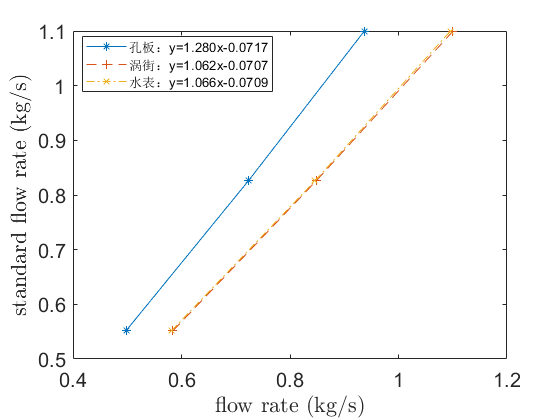
\includegraphics[width=0.6\linewidth]{figure/figure}
		\caption{标定曲线}
		\label{fig:figure}
	\end{figure}
	\subsection{误差分析}
	孔板使用法兰取压时应当满足$D > 50 mm$,雷诺数范围$8\times 10^3\sim 10^7$,而本实验使用的孔板流量计不满足以上条件,因此使用的计算流出系数的公式应当相应地修正。
	
	做空气流量标定时,由于公用气源,导致流量波动,造成误差。
	
	\subsection{多参数测量体会}
	数据采集系统精度不够,导致精度较高的流量计在AD环节产生误差,精度下降。
	
	小电流的AD采样最好使用防电磁干扰措施,如使用同轴电缆,加金属屏蔽壳等,降低采样噪声。
	\section{原始数据记录}
	\begin{figure}[H]
		\centering
		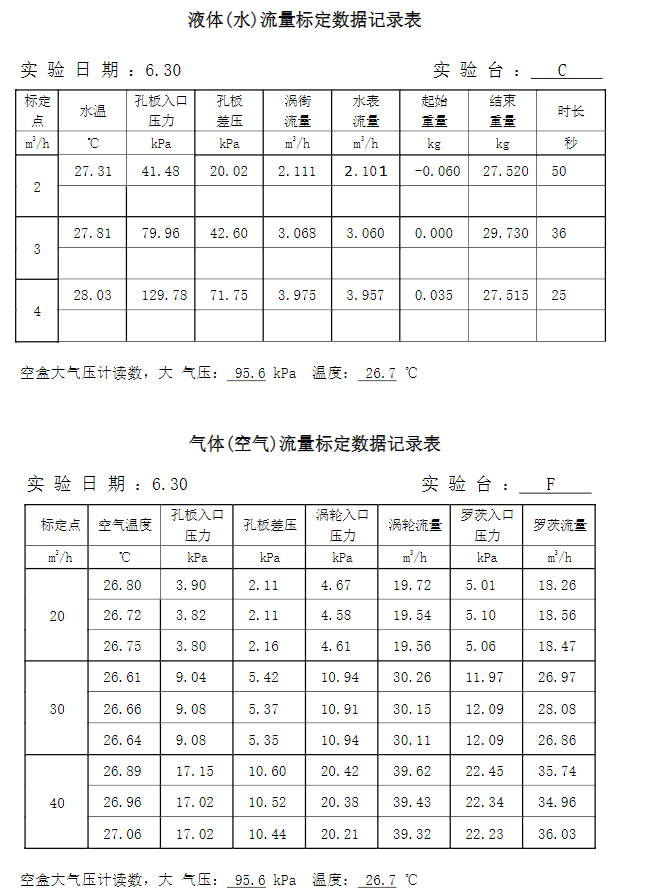
\includegraphics[width=0.7\linewidth]{figure/origin}
		\label{fig:origin}
	\end{figure}
	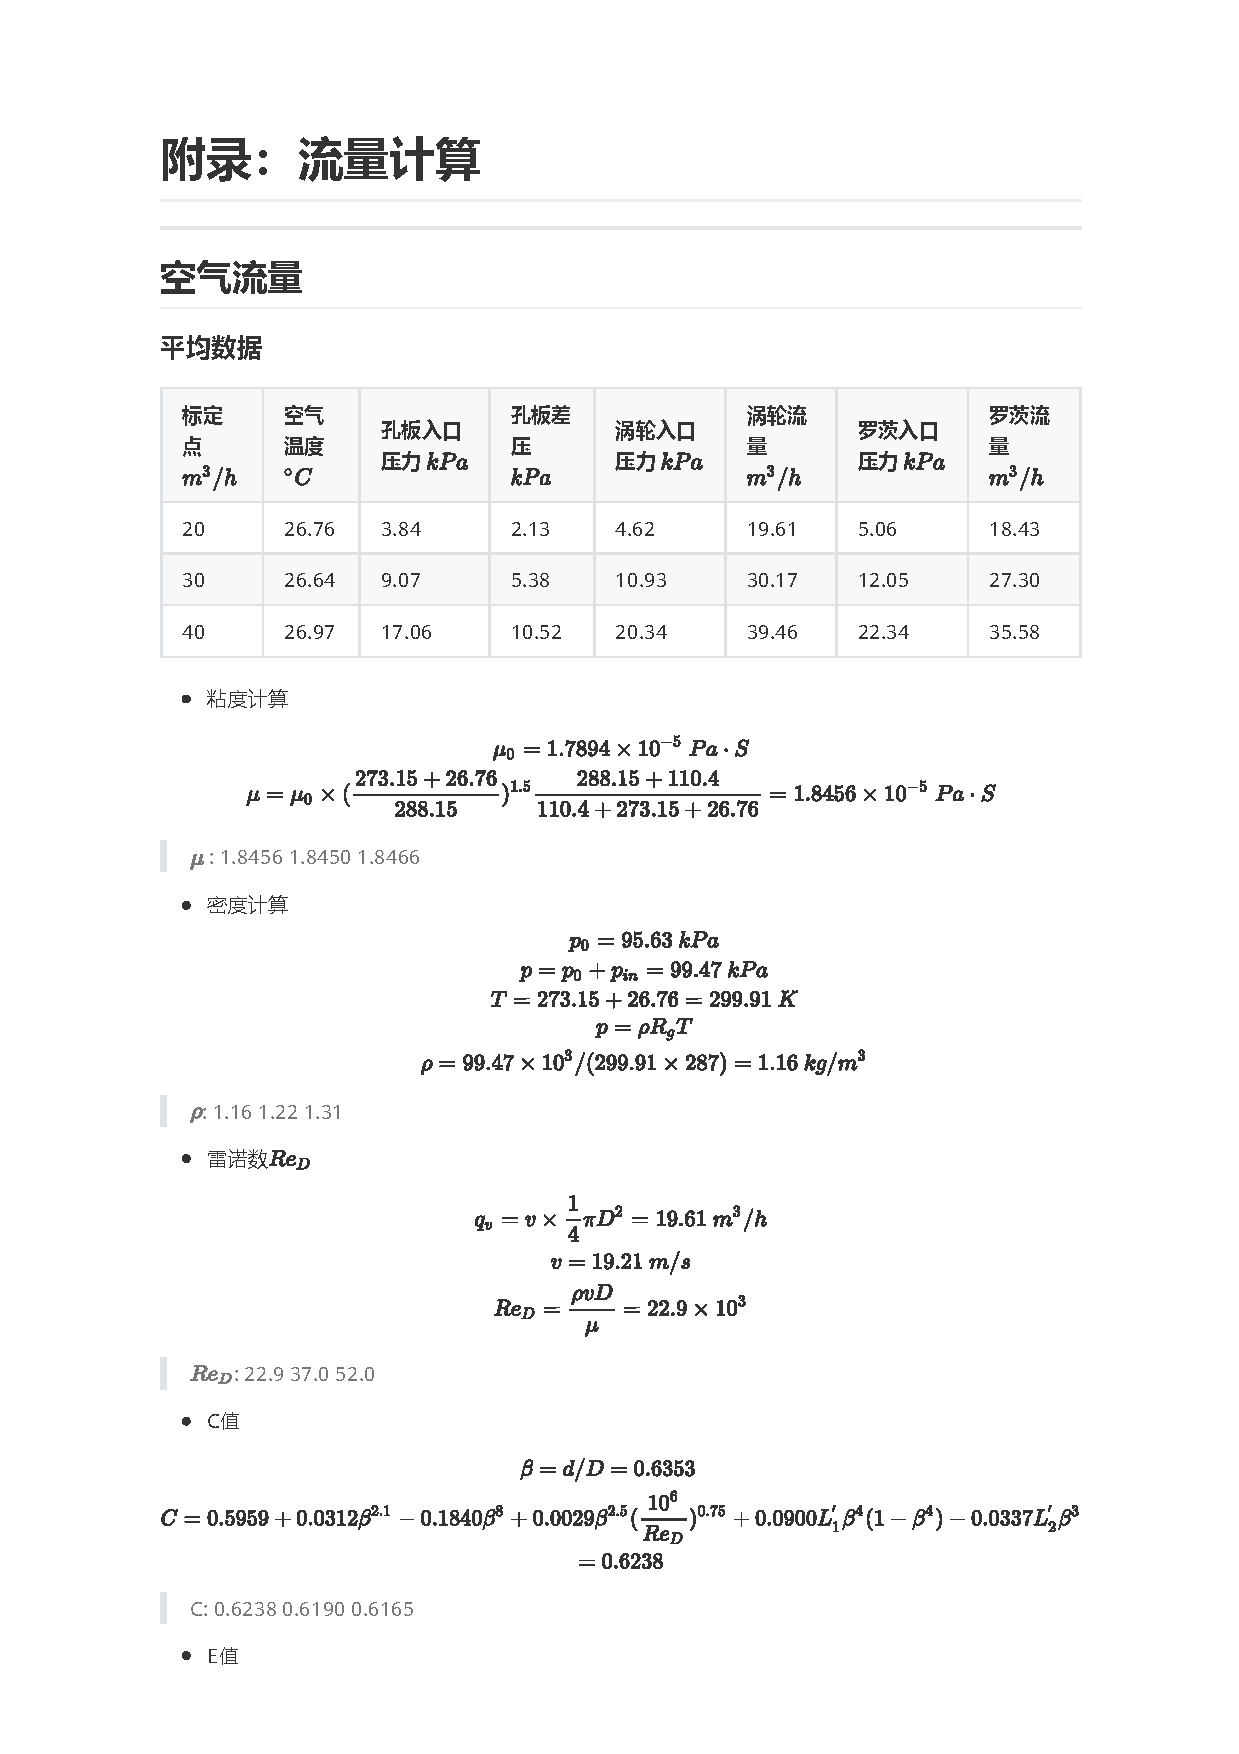
\includepdf[pages={1,2,3}]{manipulate.pdf}
\end{document}